% !TeX root = ..

\subsection{
  Стратегии проектирования маршрута режущего инструмента
  для круглых заготовок
}
\label{sect:2.2.1}

Среди часто встречающихся геометрических типов деталей
на машиностроительном производстве можно выделить заготовки,
имеющие внешний контур круглой формы.
Требуемые заготовки можно вырезать с
помощью уже известных способов резки,
например <<цепная>> резка, резка <<по замкнутому контуру>>,
однако применение рассмотренных способов резки не всегда
дает результаты, отвечающие требованиям сокращения стоимости резки.
На основании стратегии объединения однотипных заготовок
в группы разработан специальный способ резки круглых
заготовок с сокращением значений
$L_{off}, N_{pt}$
и в случае без дополнительного реза сокращении значения
$L_{on}$
при одновременном снижении
$F_{cost}$.

На рис. \ref{3-3}
приведена схема резки трех круглых заготовок
с помощью резки <<по замкнутому контуру>>,
цифрами {\it 1--3} обозначены точки врезки.
На рис.~\ref{3-1}
-- схема резки с помощью предложенного метода резки
с одной точкой врезки
(обозначенной цифрой {\it 1})
без дополнительного реза.
На обоих рисунках
буквой {\it O} обозначено начало маршрута.

\begin{figure}[H]
  \centering
  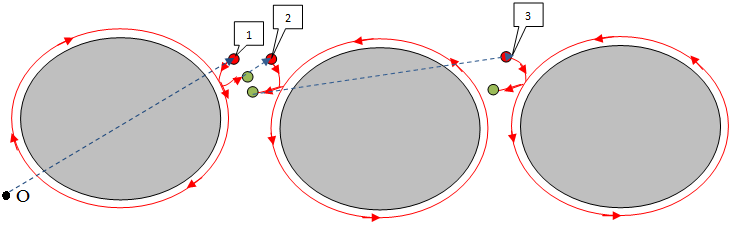
\includegraphics[width=0.9\textwidth]{3-3.png}
  \caption{
    Пример схемы резки трех круглых заготовок
    <<по замкнутому контуру>>
    }
  \label{3-3}
\end{figure}

На рис.~\ref{3-1}
цифрами от {\it 1} до {\it 5} показана последовательность
резки контуров за один сегмент,
то есть после врезания в материал режущий инструмент
на рабочем ходу переходит к вырезке участка
под номером {\it 1} первого контура,
затем без дополнительного реза режущая головка
переходит ко второму контуру и вырезает участок
контура под номером {\it 2} и т. д.
В конце режущий инструмент завершает
вырезку трех контуров с одной точкой
врезки по пятому участку первого контура и
переходит к точке выключения.
Следует обратить внимание, что в рассматриваемом
способе резки инструмент переходит от одного контура к
другому на рабочем ходу без дополнительных резов,
за счет чего сокращаются значения основных параметров резки
$L_{on}, L_{off}, N_{pt}$.

\begin{figure}[H]
  \centering
  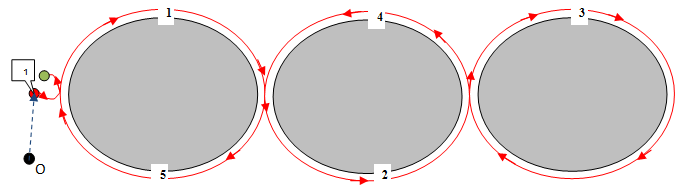
\includegraphics[width=0.9\textwidth]{3-1.png}
  \caption{
    Пример схемы резки трех круглых заготовок
    с применением специальной техники резки
    без дополнительного реза
  }
  \label{3-1}
\end{figure}

Однако в результате применения предложенного метода
резки при обработке круглых заготовок в месте <<стыковки>>
контуров возможно образование <<ступеньки>>
(см. рис.~\ref{hiccup}),
что в некоторых случаях может привести к
искажению конечной геометрии и требуемых размеров заготовки.

\begin{figure}[H]
  \centering
  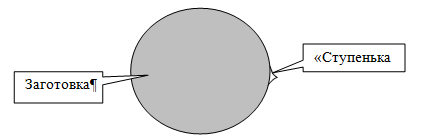
\includegraphics[width=0.7\textwidth]{hiccup.png}
  \caption{
    Возможная <<ступенька>> при обработке круглых заготовок
    с помощью специального метода резки
  }
  \label{hiccup}
\end{figure}

Как показывает практика,
при обработке круглых заготовок на
машине лазерной листовой резки с ЧПУ размеры <<ступеньки>> незначительны
(достигают десятых-сотых долей миллиметра)
и ее размеры либо попадают в требуемое поле допуска
для соответствующего размера, либо ее можно <<зачистить>>
с помощью дополнительной обработки без искажения геометрии и требуемых размеров.
Также следует отметить, что часто детали,
получаемые после лазерной обработки,
являются заготовками для дальнейших переделов с
припусками на требуемые размеры чертежа,
поэтому допускаются незначительные дефекты,
обработка которых в дальнейшем не приведет к
искажению требуемых размеров и форм конечной детали.

При размещении круглых заготовок в один ряд
либо вдоль оси $X$,
либо вдоль $Y$
возможно сокращение количества точек врезки до
$N_{pt}=1$
и сведение
$L_{off}$
к величине, равной нулю, если не считать перемещения
режущего инструмента на холостом ходу до точки врезки
для текущего ряда круглых заготовок и от точки выключения
режущего инструмента до следующей точки врезки или нулевой точки
($L_{off} \approx 0$).
В случае размещения круглых заготовок в $n$
рядов при использовании предложенного способа резки
$N_{pt}=n$.

Предложенный на рис.~\ref{3-1}
метод резки круглых заготовок в основном применим для заготовок,
которые можно объединить в один блок и применить
данную специальную технику резки без дополнительного реза.
Однако на практике возникают случаи вырезки круглых заготовок
специальным способом с дополнительным резом,
рис.~\ref{3-extra}.
Здесь аналогично
{\it O} -- начальная точка,
{it 1--5} -- ход реза.

\begin{figure}[H]
  \centering
  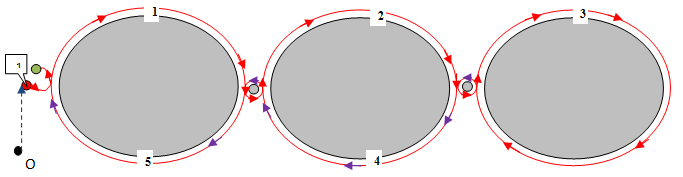
\includegraphics[width=0.9\textwidth]{3-extra.png}
  \caption{
    Пример схемы резки трех круглых заготовок
    с применением специальной техники резки с дополнительным резом
    }
  \label{3-extra}
\end{figure}

Например, на производстве возникает задача
вырезки круглых заготовок разного габаритного размера,
а также при построении маршрута перемещения режущего инструмента
на машинах термической резки с ЧПУ необходимо выполнение
технологических ограничений термической резки.
В частности, в случае необходимости выполнения условий
сокращения термических деформаций вырезку заготовок с
применением разработанной специальной техники резки
для круглых заготовок необходимо выполнять без изменения обхода контуров.
С этой целью может быть применим способ с дополнительным резом
(рис. \ref{3-extra})
во избежание повышения температуры в процессе резки контуров
в месте стыка деталей из-за острого угла
при переходе от одного контура к другому без изменения
направления обхода и во избежание образования <<ступеньки>>.
Вырезка контуров осуществляется аналогично способу,
приведенному выше
(рис.~\ref{3-3}),
однако при переходе от одного контура к другому
при необходимости возможен дополнительный рез
(при наличии деталей значительно отличающихся по размерам и смещении друг относительно друга).
В свою очередь это может привести к увеличению
$L_{on}$
на величину фактической длины дополнительных резов
$L_\text{доп}^\text{факт}$.
Поэтому в данном способе необходимо вычислять максимально допустимую длину дополнительного реза
$L_\text{доп}$
и
$L_\text{доп}^\text{факт} \leqslant L_\text{доп}$.

На рис.~\ref{3-extra}
цифрами {\it 1--3} отмечен спроектированный путь
перемещения инструмента на рабочем ходу при прямом обходе контуров,
цифрами {\it 4, 5} -- обратный ход режущего инструмента
при завершении вырезки трех деталей с
применением специальной техники резки.

Согласно предложенному методу режущая головка
после врезания в материал обходит по часовой
стрелке первый участок контура
(под номером {\it 1}),
после чего, меняя направление обхода против
часовой стрелки,
совершает дополнительный рез и
переходит к вырезке участка
(под номером {\it 2})
второго контура по часовой стрелке и т. д.
Пока режущий инструмент не завершит
вырезку полного контура с номером {\it 3},
после чего режущая головка совершает обратный обход
оставшихся невырезанных частей контуров под номерами
{\it 4} и {\it 5}.
Таким образом, можно вырезать заготовки разных размеров,
объединенных в блоки, и внутри каждого блока реализовать
вырезку нескольких контуров с помощью одной точки врезки.
При этом дополнительный рез может быть выполнен по дуге
либо по прямой в зависимости от размера внешнего контура заготовок.

С целью оценки эффективности в результате применения
разработанных специальных способов резки рассмотрим
пример резки круглых заготовок двумя вышеописанными
методами на машине лазерной листовой резки
{\it ByStar 3015} с ЧПУ.
Для этого были разработаны две раскройные карты,
на которых размещены 69 и 58 заготовок,
имеющих круглый наружный контур.

На рис.~\ref{circles-a}
и~\ref{circles-b}
приведен маршрут резки
круглых заготовок одного размера без дополнительного реза,
на рис.~\ref{circles-c}
и~\ref{circles-d} -- с дополнительным резом.
Во всех случаях маршрут резки начинается из
левого нижнего угла листа.

Полученные результаты сравнивались с результатами
резки <<по замкнутому контуру>> и приведены в
табл.~\ref{circles}
на с.~\pageref{circles}.
Расчет был произведен для листового материала
{\it 12Х18Н10Т}
$\Delta$ = 1 и 5 мм.

На рис. \ref{circles-d}
разными цветами обозначены блоки деталей,
для которых реализована резка без дополнительного реза.
В частности, в нижней  части раскройной карты
может быть выделена
группа из 10 круглых заготовок и одного кольца.

\begin{figure}[H]
  \centering
  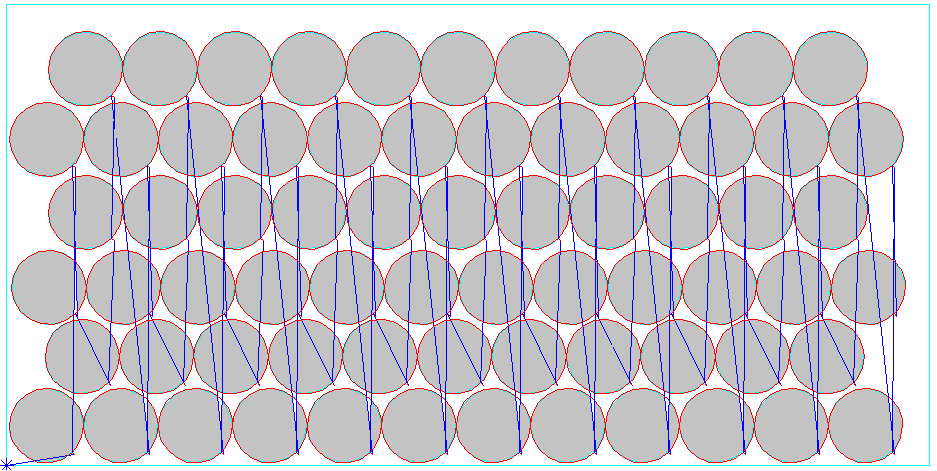
\includegraphics[width=0.9\textwidth]{circles-a.png}
  \caption{
    Пример маршрута резки круглых заготовок
    c~применением резки
    <<по~замкнутому контуру>>
  }
  \label{circles-a}
\end{figure}

\begin{figure}[H]
  \centering
  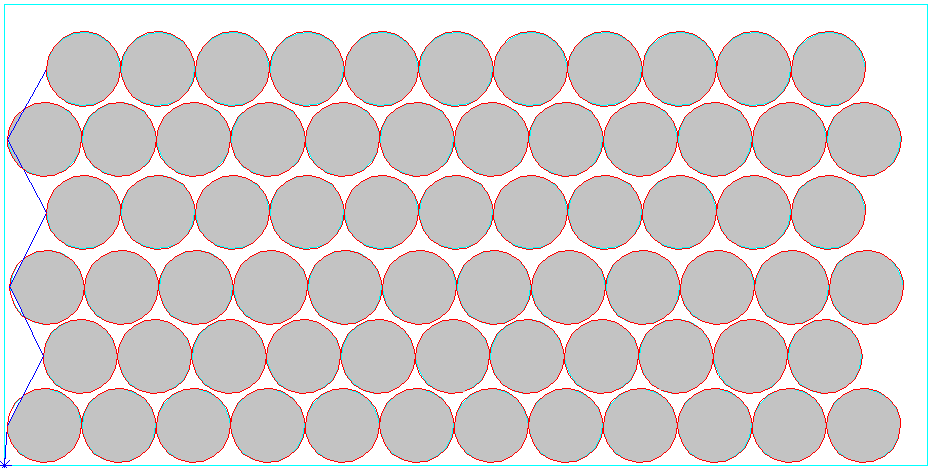
\includegraphics[width=0.9\textwidth]{circles-b.png}
  \caption{
    Пример маршрута резки круглых заготовок
    c~применением метода резки
    без~дополнительного реза
  }
  \label{circles-b}
\end{figure}

Размеры заготовок отличаются незначительно,
поэтому есть возможность реализовать резку блока из 11 деталей с
помощью одной точки врезки и без дополнительного реза.
В  верхней части той же раскройной карты выделен блок из шести деталей,
вырезаемых с одной точкой врезки, при этом заготовки,
выделенные фиолетовым цветом, вырезаются без дополнительного реза,
но при переходе к серым заготовкам меньшего размера необходимо
вырезку осуществить с дополнительным резом.
Отметим, что
дальнейшая вырезка трех серых заготовок
осуществляется без дополнительного реза.

\begin{table}[H]
  \caption{
    Результаты расчета стоимость резки раскройного плана
    для~круглых заготовок
    с~применением специальных способов резки
    }
  \label{circles}
  \centering
  \small
  \begin{tabular}{c *{8}{ | c }}
    \hline
    Марка & $\Delta$ & Резка
      & \shortstack{$L_{on}$, \\ м}
      & \shortstack{$L_{off}$, \\ м}
      & $N_{pt}$
      & \shortstack{$F_{cost}$,\\ руб}
      & \%
      & \shortstack{$L_\text{доп}^\text{факт}$,\\ м} \\
    \hline
    \hline
    \multirow{8}{*}{\rotatebox{90}{12Х18Н10Т}} & \multirow{4}{*}{1 мм} & Стандартная & 54,7 &	43,07	& 69 & 1552,92 & \multirow{2}{*}{15,6} &	\multirow{2}{*}{--} \\
    \cline{3-7}
    & & Без доп, реза & 52,02 &	0,7 & 6 & 1310,05 & \\
    \cline{3-9}
    & & Стандартная   & 46,14 & 18,78 & 58 & 1302,08 & \multirow{2}{*}{6,88} & \multirow{2}{*}{0,16} \\
    \cline{3-7}
    & & С доп, резом  & 46,3  & 5,43  & 23 & 1212,43 & \\
    \cline{2-9}
    & \multirow{4}{*}{5 мм} & Стандартная & 54,7 &	43,07	& 69 & 12154,8 & \multirow{2}{*}{14,3} &	\multirow{2}{*}{--} \\
    \cline{3-7}
    & & Без доп, реза & 52,02 &	0,7 & 6 & 10417,2 & \\
    \cline{3-9}
    & & Стандартная   & 46,14 & 18,78 & 58 & 10241,6 & \multirow{2}{*}{6,2} & \multirow{2}{*}{0,16} \\
    \cline{3-7}
    & & С доп, резом  & 46,3  & 5,43  & 23 & 9607,08 & \\
    \hline
  \end{tabular}
\end{table}

\begin{figure}[H]
  \centering
  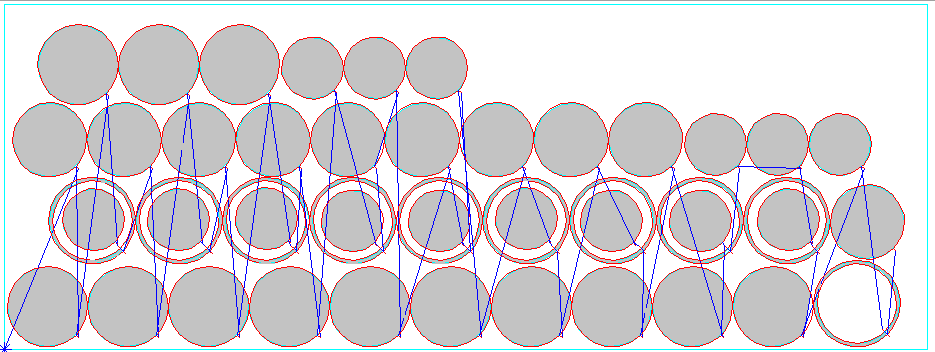
\includegraphics[width=0.9\textwidth]{circles-c.png}
  \caption{
    Пример маршрута резки круглых заготовок разного размера
    c~применением резки
    <<по~замкнутому контуру>>
    }
  \label{circles-c}
\end{figure}

\begin{figure}[H]
  \centering
  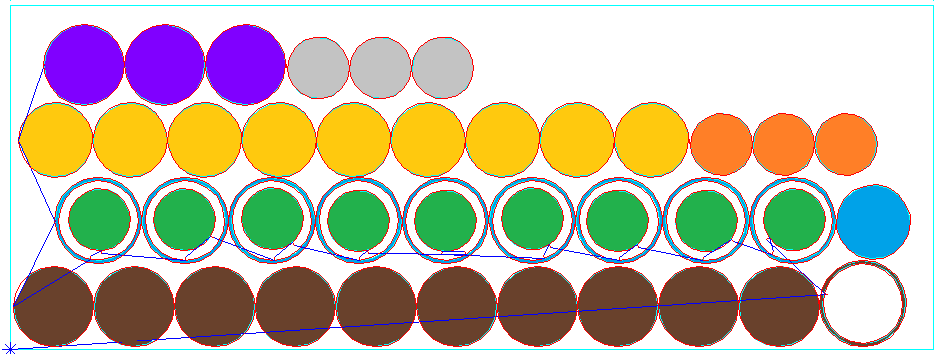
\includegraphics[width=0.9\textwidth]{circles-d.png}
  \caption{
    Пример маршрута резки круглых заготовок разного размера
    c~применением специальной техники резки
    }
  \label{circles-d}
\end{figure}

По результатам анализа приведенных
в~табл.~\ref{circles}
данных, можно сделать следующие выводы.

\begin{enumerate}
\item
Применение специального метода резки круглых заготовок
без дополнительного реза
(рис.~\ref{circles-b})
приводит к сокращению количества точек врезок до 90 \%
и длины перемещений инструмента на холостом ходу до 98 \%
по сравнению с резкой по <<замкнутому контуру>>.
При проведении ряда экспериментов значение $N_{pt}$
сокращается в среднем на 60 \%, значение $L_{off}$ -- на 65 \%.
При этом стоимость обработки раскройной карты в среднем сокращается на 15 \%.

\item
Применение резки с дополнительным резом
(рис.~\ref{circles-d})
приводит в среднем к сокращению количества точек врезок на 60 \%,
а длина перемещений инструмента на холостом ходу сокращается на 70 \%
по сравнению с резкой <<по замкнутому контуру>>.
В свою очередь, стоимость обработки сокращается на 7 \%.
При этом следует отметить,
что по причине наличия внутренних контуров
наблюдается снижение эффективности применения
предложенных технологий.

\item
В случае применения резки с дополнительным резом необходимо рассчитать
$L_\text{доп}^\text{факт}$
и
$L_\text{доп}$
согласно (\ref{l-dop}) и (\ref{l-fact-dop}).
\end{enumerate}
